\documentclass{article}
\usepackage[utf8]{inputenc}
\usepackage{amssymb}
\usepackage{amsthm}
\usepackage{amsmath}
\usepackage{epic}
\usepackage{eepic}
\usepackage{paralist}
\usepackage{listings}
\usepackage{graphicx}
\usepackage{algorithm,algorithmic}
\usepackage{tikz}
\usepackage{xcolor,colortbl}
\usepackage{wrapfig}
\usepackage{xcolor}
\usepackage[margin = 1 in]{geometry}


%New colors defined below
\definecolor{codeblue}{rgb}{0,0.1,0.9}
\definecolor{codegreen}{rgb}{0,0.5,0}
\definecolor{codegray}{rgb}{0.5,0.5,0.5}
\definecolor{codeyellow}{rgb}{0.5,0.5,0}
\definecolor{backcolour}{rgb}{1.0,1.0,1.0}

%Code listing style named "mystyle"
\lstdefinestyle{mystyle}{
backgroundcolor=\color{backcolour},   commentstyle=\color{codeyellow},
keywordstyle=\color{codeblue},
numberstyle=\tiny\color{codegray},
stringstyle=\color{orange},
basicstyle=\ttfamily \normalsize,
breakatwhitespace=false,         
breaklines=true,                 
captionpos=b,                    
keepspaces=true,                 
lineskip=0.2em,
numbers=left,                    
numbersep=5pt,                  
showspaces=false,                
showstringspaces=false,
showtabs=false,                  
tabsize=2
}

%"mystyle" code listing set
\lstset{style=mystyle}


\title{CS5220: Shallow Water Project}
\author{Cheng Perng Phoo, Robert Stephany, Junyoung Lim}
\date{November 3, 2020}

\begin{document}

\maketitle

\section{Introduction}

In this project, we have tried various ways to optimize and tune the implementation of a finite volume solver for 2D hyperbolic PDEs via a high-resolution finite difference scheme (TODO: cite a reference to Jiang and Tadmor). Our approaches are built upon two central themes: subdomain partitioning and parallelization using OpenMP. Based on the performance analysis, the best tuning we have achieved has (TODO: one-two lines summary of the performance result).

\section{Discussion: Compilation Details}

Although we used different environments (Mac, Ubuntu, Arch) for local testing and debugging, the profiling and performance analysis have been done on Graphite. Here in this section, we discuss the compilation configurations we used.

We used the GCC x.x.x (TODO: @Cheng can you specify any details about the compiler version here if there is any?) compiler provided by Graphite. The four flags that we used for the compilation are the following:
\begin{itemize}
	\item \texttt{-O3} --- Performs more aggressive optimization than \texttt{-O2} used by default.
	\item \texttt{-ffast-math} --- Enables the compiler to reorder operations that may not actually be associative.
	\item \texttt{-fopenmp} --- Enables the OpenMP directive \texttt{\#pragma omp} in our C code for shared memory parallel processing.
	\item \texttt{-march=native} --- Optimizes the code for the specific machine architecture.
\end{itemize}

\section{Discussion: Subdomain Partitioning}

\subsection{Overview}
The first approach is to partition the grid data, $U_G$, into $N$ subgrids, $U_i$, each with its own start and end indices for both $x$ (horizontal) and $y$ (vertical) direction. In this report and our implementation, we will often refer to $U_i$ as a local grid, and $U_G$ as the global grid. Assume that each thread will handle each $U_i$ in a parallel manner. The overview below will overlook any parallelization aspect of the logic since more details about parallelization through OpenMP will come in the next section.

Before processing each $U_i$, we first apply periodic boundary conditions to $U_G$ (this is the same as the originally provided work). This order of operation ensures that the ghost cells of $U_G$ can be easily pulled into those of each $U_i$. Then we can safely apply boundary conditions to each $U_i$ by copying over the ghost cells from $U_G$ to $U_i$.

Once boundary conditions are applied, we compute the maximum wave speed in the $x$ and $y$ direction and determine $dt$. Unlike the original work, in which $dt$ is computed directly using $U_G$, we need to compute the maximum $x$ and $y$ velocities from each local grid and determine $dt_i$ for each $U_i$. Once all the computations are done, we determine $dt$ to be $\min\{dt_i\}_{i=1}^N$.

The rest of the main loop logic is the same as the original work, except that we need to make sure that copy the boundary of each local grid to the corresponding location in the global grid. Then proceed to the next iteration of the loop only after all the boundaries are copied over.

\subsection{Implementation Details}

Only some of the noteworthy code snippets, which will help understanding the implementation details, are exposed in this section.

In order to apply the idea of subdomain partitioning, we need to determine $N$, the number of partitions to create. To generalize our logic, we dynamically determine the number of partitions at runtime by detecting $p$, the number of threads running, and let $N = p$.


\begin{lstlisting}[language=C]
// ldriver_parallel.c
// First get the number of threads from the environment
// If the number of threads is null, then set the number of threads to 1
char* s = getenv("OMP_NUM_THREADS");

int num_threads = 0;
if (s != NULL) {
    num_threads = atoi(s);
} 

if (num_threads == 0) {
    num_threads = 1;
}

printf("Number of threads: %d\n", num_threads);
const int n_rows = num_threads;
const int n_cols = 1;
\end{lstlisting}

\texttt{n\_row} and \texttt{n\_col} are used to compute the location (\texttt{nx\_local} and \texttt{ny\_local}) in $U_G$ that corresponds to each $U_i$. Note that $\texttt{n\_row} = N$ and $\texttt{n\_col} = 1$, because we are exploiting the fact that matrices follow row major ordering in our code. Initialize each $U_i$ as shown below.

\begin{lstlisting}[language=C]
// ldriver_parallel.c
float* U_local = sim_local->U;
float* U = sim -> U;
for(int k = 0; k < 3; ++k) {  // 3 = nfield
  for(int iy = 0; iy < ny_local; ++iy) {
    for(int ix = 0; ix < nx_local; ++ix) {
      U_local[central2d_offset(sim_local, k, ix, iy)]
        = U[central2d_offset(sim, k, xlow_local + ix, ylow_local + iy)];
    }
  }
}
\end{lstlisting}

\texttt{stepper\_parallel.c} contains the main logic described in the overview. In addition to the provided functions, we introduce three new functions, each with the following functionalities:

\begin{itemize}
	\item \texttt{central2d\_local\_BC} --- Applies boundary conditions to from $U_G$ to $U_i$.
	\item \texttt{central2d\_local\_to\_global} --- Copies the boundary of $U_i$ back to $U_G$.
	\item \texttt{central2d\_U\_to\_global\_U} --- Copies the canonical cells of $U_i$ back to corresponding locations in $U_G$.
\end{itemize}

\section{Discussion: OpenMP Parallelization}

The aforementioned subdomain partitioning involves handling $N$ disjoint partitions, which means each of them can be handled in a parallel manner. \texttt{\#pragma omp} directives are used to ensure proper setup of parallel processing of each thread.

As soon as we figure out $p$, the number of threads, we can initialize each $U_i$ and its corresponding location in the global grid $U_G$ from the thread number assuming row-wise partitioning. It's necessary to set the barrier before running a simulation so that all threads finish up their $U_i$ initialization.

\begin{lstlisting}[language=C]
// ldriver_parallel.c
#pragma omp parallel num_threads(n_rows*n_cols)
{
    // use omp_get_thread_num() to compute the sub grid location
    // call central2d_init(...)
    // initialize U_i, as shown in Section 3
    
    // wait for all threads to set up their local arrays.
    #pragma omp barrier
    ...
}
\end{lstlisting}

Once all threads are ready with their initialization phase, run the simulation for each frame. By the time it needs to compute $dt$ from the maximum $x$ and $y$ velocities as described above, we can parallelize the operation by letting the first-arriving thread to create a shared buffer (with a single directive). Then each thread $T_i$ arrives and writes the minimum between $dt_i$ and the value already stored in the shared buffer. Wait until all threads are completed, and move on.

\begin{lstlisting}[language=C]
// inside central2d_xrun(...) of stepper_parallel.c
    ...
    // calculate dt_local using the data on our partition.

    // Initialize the shared buffer, because the buffer may contain 0.
    #pragma omp single
    {
      shared_buffer[0] = dt_local;
    }

    // Now, each thread writes its data to shared_buffer one by one.
    #pragma omp critical
    {
      shared_buffer[0] = fmin(dt_local, shared_buffer[0]);
    }
    #pragma omp barrier
    ...
\end{lstlisting}

Before exiting the main loop, we copy boundary of $U_i$ back to $U_G$. This needs to be done because at the start of the next time step, we're going to apply periodic boundary conditions, and that will only give the result we want if each thread has written its cells into $U_G$.

\begin{lstlisting}[language=C]
// inside central2d_xrun(...) of stepper_parallel.c
    ...
    // copy boundary of U to corresponding entries of U global using central2d_local_to_global(...)
    #pragma omp barrier
    ...
\end{lstlisting}

Because of this last barrier directive in \texttt{central2d\_xrun}, we can use one of the time measurement to get an elapsed time. Have one section for proving the correctness of our solution, and the other one for writing $U_i$ to memory.

\begin{lstlisting}[language=C]
// ldriver_parallel.c
#pragma omp parallel num_threads(n_rows*n_cols)
{
    ...
    #pragma omp barrier
    
    for (int i = 0; i < frames; ++i) {
        // measure time elapsed from central2d_run(...)
        
        #pragma omp sections {
            #pragma omp section {
              // run out diagnostic on U_i by running solution_check(...)
            }
            #pragma omp section {
              //  write a frame of U to memory by running viz_frame(...);
            }
        }
    }
    ...
}
\end{lstlisting}

\section{Performance Analysis}

Keep the same notation as above, where$p$ is the number of threads, and assume each thread is uniquely associated to a processor.

\subsection{Strong Scaling}

We performed strong scaling on Graphite. In particular, we set the problem size to be $nx = ny = 1000$ and ran our implementation for $p = 1, 2, 3, \ldots, 10$. We compute the speedup as $T_{serial} / T_{parallel}$ where $T_{serial}$ was benchmarked using the initial code released to us. We plotted the speedup against the number of threads in figure 1. Our strong scaling plot demonstrated a close to linear scaling for the number of threads less than or equal to 5 but the speedup tapered off as increased the number of threads. Our finding aligned with Amdahl’s Law, i.e, there always exists some code that is inherently serial and hard to parallelize and those serial work upper bound the speedup of parallel code.

\subsection{Weak Scaling}
To run weak scaling, we had to scale the problem size with respect to the number of threads such that the amount of work per processor is identical for each thread. However, this will be hard to achieve if we want to maintain a square grid data. For instance, suppose we conduct weak scaling on a single thread on a grid of size $h \times h$, then to run weak scaling with 2 threads, we have to run on a grid of size $2h \times h$ or $h \times 2h$ which is no longer a square grid. As such, we conducted two variants of weak scaling:

\begin{enumerate}
    \item Maintaining the square grid
    
    To make sure that we could conduct weak scaling on a square grid data, we made a compromise by setting the grid’s height and width to be $\lfloor \sqrt{p} \rfloor \times 500$. We plot the scaled speedup in Figure 2. The scaled speedup hovered around 2 for $p \ge 2$ (the trendline did show that the scaled speedup increased linearly with respect to $p$ but the effect of $p$ is negligible for small $p$). Our finding was aligned with Gustafson’s Law, i.e, the scaled speedup is $O(p)$.
    
    \item Keeping the amount of work per processor identical
    
    To ensure similar workload for each processor, we conducted weak scaling on grid data of size $500 \times 500p$ (violating the square grid assumption) so that each thread would operate on a grid data of size $500 \times 500$. We plotted the scaled speedup in Figure 3. Again, we found that the scaled speedup hovered around 2 for $p \ge 2$ with linear dependence with the number of threads. Our finding was yet again consistent with Gustafson’s Law.  
\end{enumerate}

\section{Attempts That Didn't Work}

\subsection{Using OpenMP with MPI}

We attempted using MPI along with OpenMP but we were not able to compile our code so we ended up simulating MPI using openmp. 

\subsection{Naively Inserting \text{\#pragma omp parallel}}

We started the project by profiling the serial code provided using gprof (see Figure 4) and tried parallelizing a few functions using OpenMP. In particular, we tried adding \texttt{\#pragma omp parallel for} in three functions: \texttt{central2d\_correct\_sd}, \texttt{shallow\_2dv\_flux} and \texttt{shallow\_2dv\_speed} but we ended up with an implementation that is significantly worse than the serial code.

\begin{figure}[h!]
	\centering
	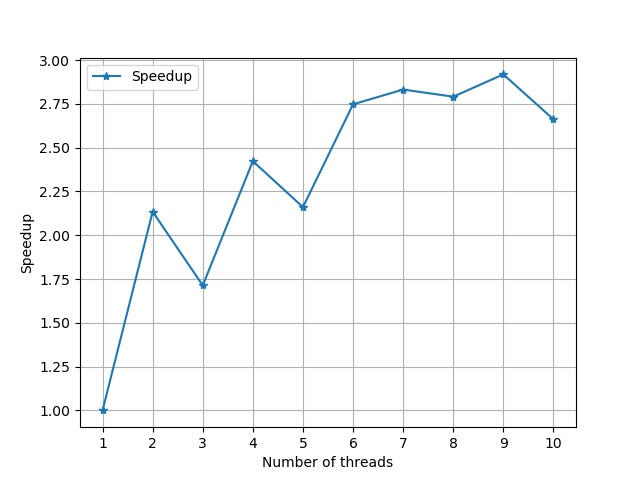
\includegraphics[width=0.8\columnwidth]{../strong_scaling.jpg}
	\caption{Speedup for Strong Scaling Study}
	\label{fig:strong_scaling}
\end{figure}

\begin{figure}[h!]
	\centering
	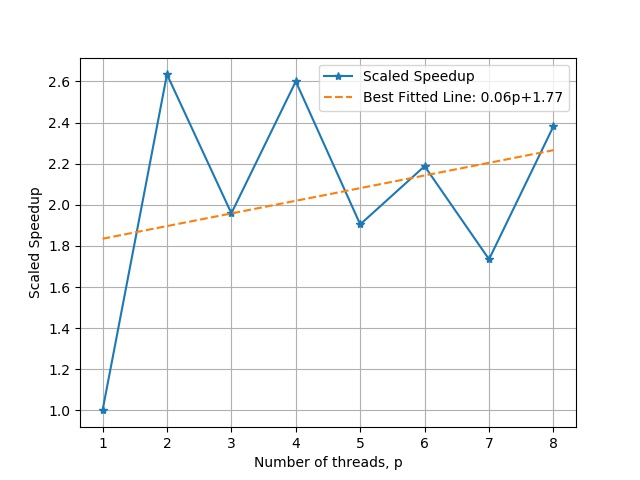
\includegraphics[width=0.8\columnwidth]{../weak_scaling.jpg}
	\caption{Speedup for Weak Scaling (Square Grid)}
	\label{fig:weak_scaling}
\end{figure}

\begin{figure}[h!]
	\centering
	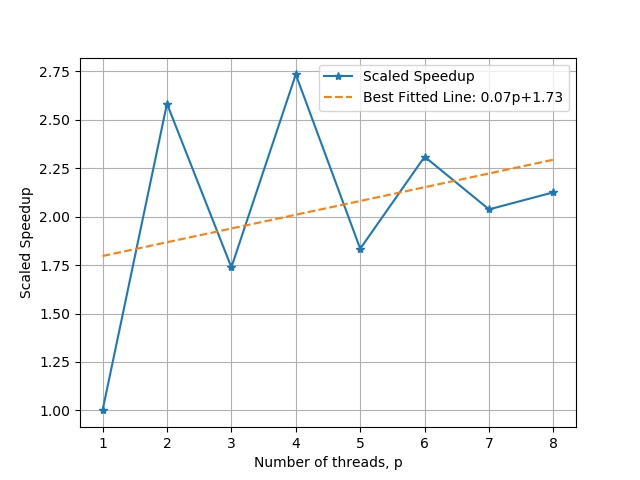
\includegraphics[width=0.8\columnwidth]{../weak_scaling_v2.jpg}
	\caption{Speedup for Weak Scaling (Constant Workload for Processor)}
	\label{fig:weak_scaling_v2}
\end{figure}

TODO: add Output from Gprof diagram.

\section{Conclusion}

TODO: write a conclusion.

\end{document}
